\chapter{ARACNE-structure learning}
\label{ch-aracne}

This chapter
is based on
Ref.\cite{aracne}.

The ARACNE algo
is an algo for learning the structure
of a bnet from data.
The algo
considers data samples
for $n$ random variables
$(x_i)_{i=0, 1, \dots, n-1}$,
and estimates the mutual
information $MI_{i,j}=H(\rvx_i:\rvx_j)$ between
every pair of nodes.
The set $UG$ is initialized to
contain all the edges of a fully connected
undirected graph.
Next the algo
removes from $UG$
every edge with $MI_{i,j}<\eps$
for some threshold $0<\eps<<1$.
Then the algo examines every
triplet of edges
in $UG$, and marks for removal 
the edge of the triplet
with the smallest MI.
Finally,
the algo removes from $UG$  all
edges marked for removal.
 Each triplet is analyzed
irrespective of whether its edges
 have been marked for
removal when considering a prior triplet.
Thus the network constructed by the 
algorithm is independent of the
 order in which the triplets are examined.
Some of the unoriented edges in
$UG$
can be given an orientation
using the same techniques
used to orient edges
in constraint based structure
learning (see Chapter \ref{ch-struc-learn}).



Ref.\cite{aracne} incorrectly claims that
removing the smaller of 3 MI's
is ``an application" of the Data Processing 
Inequality (DPI)
of Shannon Information Theory. 
See Chapter \ref{ch-mchain}
for more info about DPI.
Note that DPI is
only valid for a Markov chain,
and not all
 triplets of random variables
are in a Markov chain.
Removing the smaller of 
3 numbers does not require DPI.

\begin{figure}[h!]
\centering
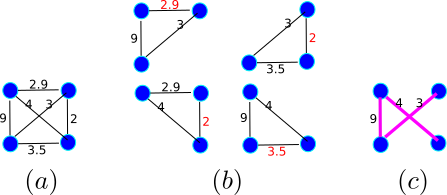
\includegraphics[width=4in]
{aracne/aracne.png}
\caption{
An example where the ARACNE algo 
gives a Chow-Liu tree.
$(a)$ Fully connected 
undirected graph with
 weights $MI_{i,j}$
along the edges.
$(b)$ All 4 possible triplets of edges
with nonzero weights.
Edges marked for removal 
have their weights
printed in red.$(c)$
Final structure.} 
\label{fig-aracne}
\end{figure}


Fig.\ref{fig-aracne}
gives an example 
of the application
of the ARACNE algo.

See Chapter \ref{ch-chow} on 
Chow-Liu trees (CLT).
A CLT is just
a  maximum spanning tree
where the weights are 
mutual informations 
 $MI_{i,j}$
estimated from data.

Sometimes, the outcome
of the ARACNE algo is a CLT.
For example,
Fig.\ref{fig-aracne}
$(a)$
was considered
in Chapter \ref{ch-chow}
on CLTs, and
the CLT algo
also
gave 
Fig.\ref{fig-aracne}
$(c)$ as the final structure.

According to Ref.\cite{aracne}, the 
 ARACNE algo sometimes 
yields  a polytree (i.e., 
a connected graph with no loops).
It may even  
yield a structure with loops.
Hence, it does not always yield a CLT.

By breaking all cliques (i.e., fully
connected subgraphs)
with 3 edges, ARACNE 
breaks all cliques with  
3 or more edges. 
However, cliques are 
not uncommon in Nature,
especially 3 edge cliques. 
Cliques become less likely in Nature 
the bigger the number of edges they have
{\it after} 3.
Therefore, a nice  
generalization of ARACNE
would be to list all 
4 edge cliques,
and break 
them by eliminating their edge
with the smallest MI.
This will
have the effect of breaking
all cliques with 
4 or more edges
but keeping 3 edge cliques.
One could also break
some, not all, of the 3 edge cliques,
starting with the ones with the smallest
sum of MI's for the 3 edges.
Let $\beta$ stand for banned clique
size.  Then
the current ARACNE has 
$\beta=3$.
We are suggesting that a $\beta$ of
4 might be more likely
to occur in Nature.

